\chapter{Use Cases for the Extension Method} \label{chap:usecases}
Evaluation of our SDOG modifications is done quantitatively through an analysis of volume preservation and compactness (\cref{chap:4:results}) and runtime performance of coding algorithms (\cref{chap:7:runtime}).
For the grid extension method---as there is no single resulting 3D DGGS to analyze---we perform evaluation through a series of use cases for 3D DGGS's.
These use cases are not state-of-the-art implementations; however, they demonstrate the robustness and versatility of the approach and its ability to support different target applications, data sets, and input DGGS's.
For each use case, we chose an input DGGS and parameters for the system that resulted in a 3D DGGS with desirable properties for said application.
The data encodings in these use cases are all defined using the fundamental operations of the 3D DGGS.


The content of this chapter is taken from our \textit{IJGL} article~\cite{ulmer2020general}.
Additional details on each use case have been added, along with an expanded description of implementation details.


\section{Use Cases}
Three use cases were chosen to evaluate the method: aircraft and satellite paths, atmospheric properties, and urban planning.
To create the use cases, we have implemented the extension method as a C++ class.
This 3D DGGS class takes an input DGGS as well as values for the target aspect ratio ($a$), exponent for the radial mapping ($t$), and the radial range of the grid ($R_\mathrm{max}$) as input during construction.
Further implementation details are provided in \cref{chap:8:impl}.


\subsection{Aircraft and Satellite Paths} \label{chap:8:sats}
The first use case we examine is tracking aircraft and spacecraft trajectories, such as commercial and private flights, drones, satellites, and rockets.
Such a system could be used to increase the efficiency of collision queries using the hierarchy of the grid system, similar to the approaches of~\cite{miao2019low, zhai2019collision}.
The main benefit our 3D DGGS's would offer over existing grids for such a system is the ability to have cells located at low and high altitudes in the same resolution have close to equal shape and size.
This use case clearly demonstrates the ability for our 3D DGGS's to support datasets with arbitrarily large ranges of altitudes; in this case, up to 35,000~km.
It also shows how geospatial data represented as vector polylines is encoded and rasterized in a 3D DGGS.


\begin{figure}[ht!]
	\centering
	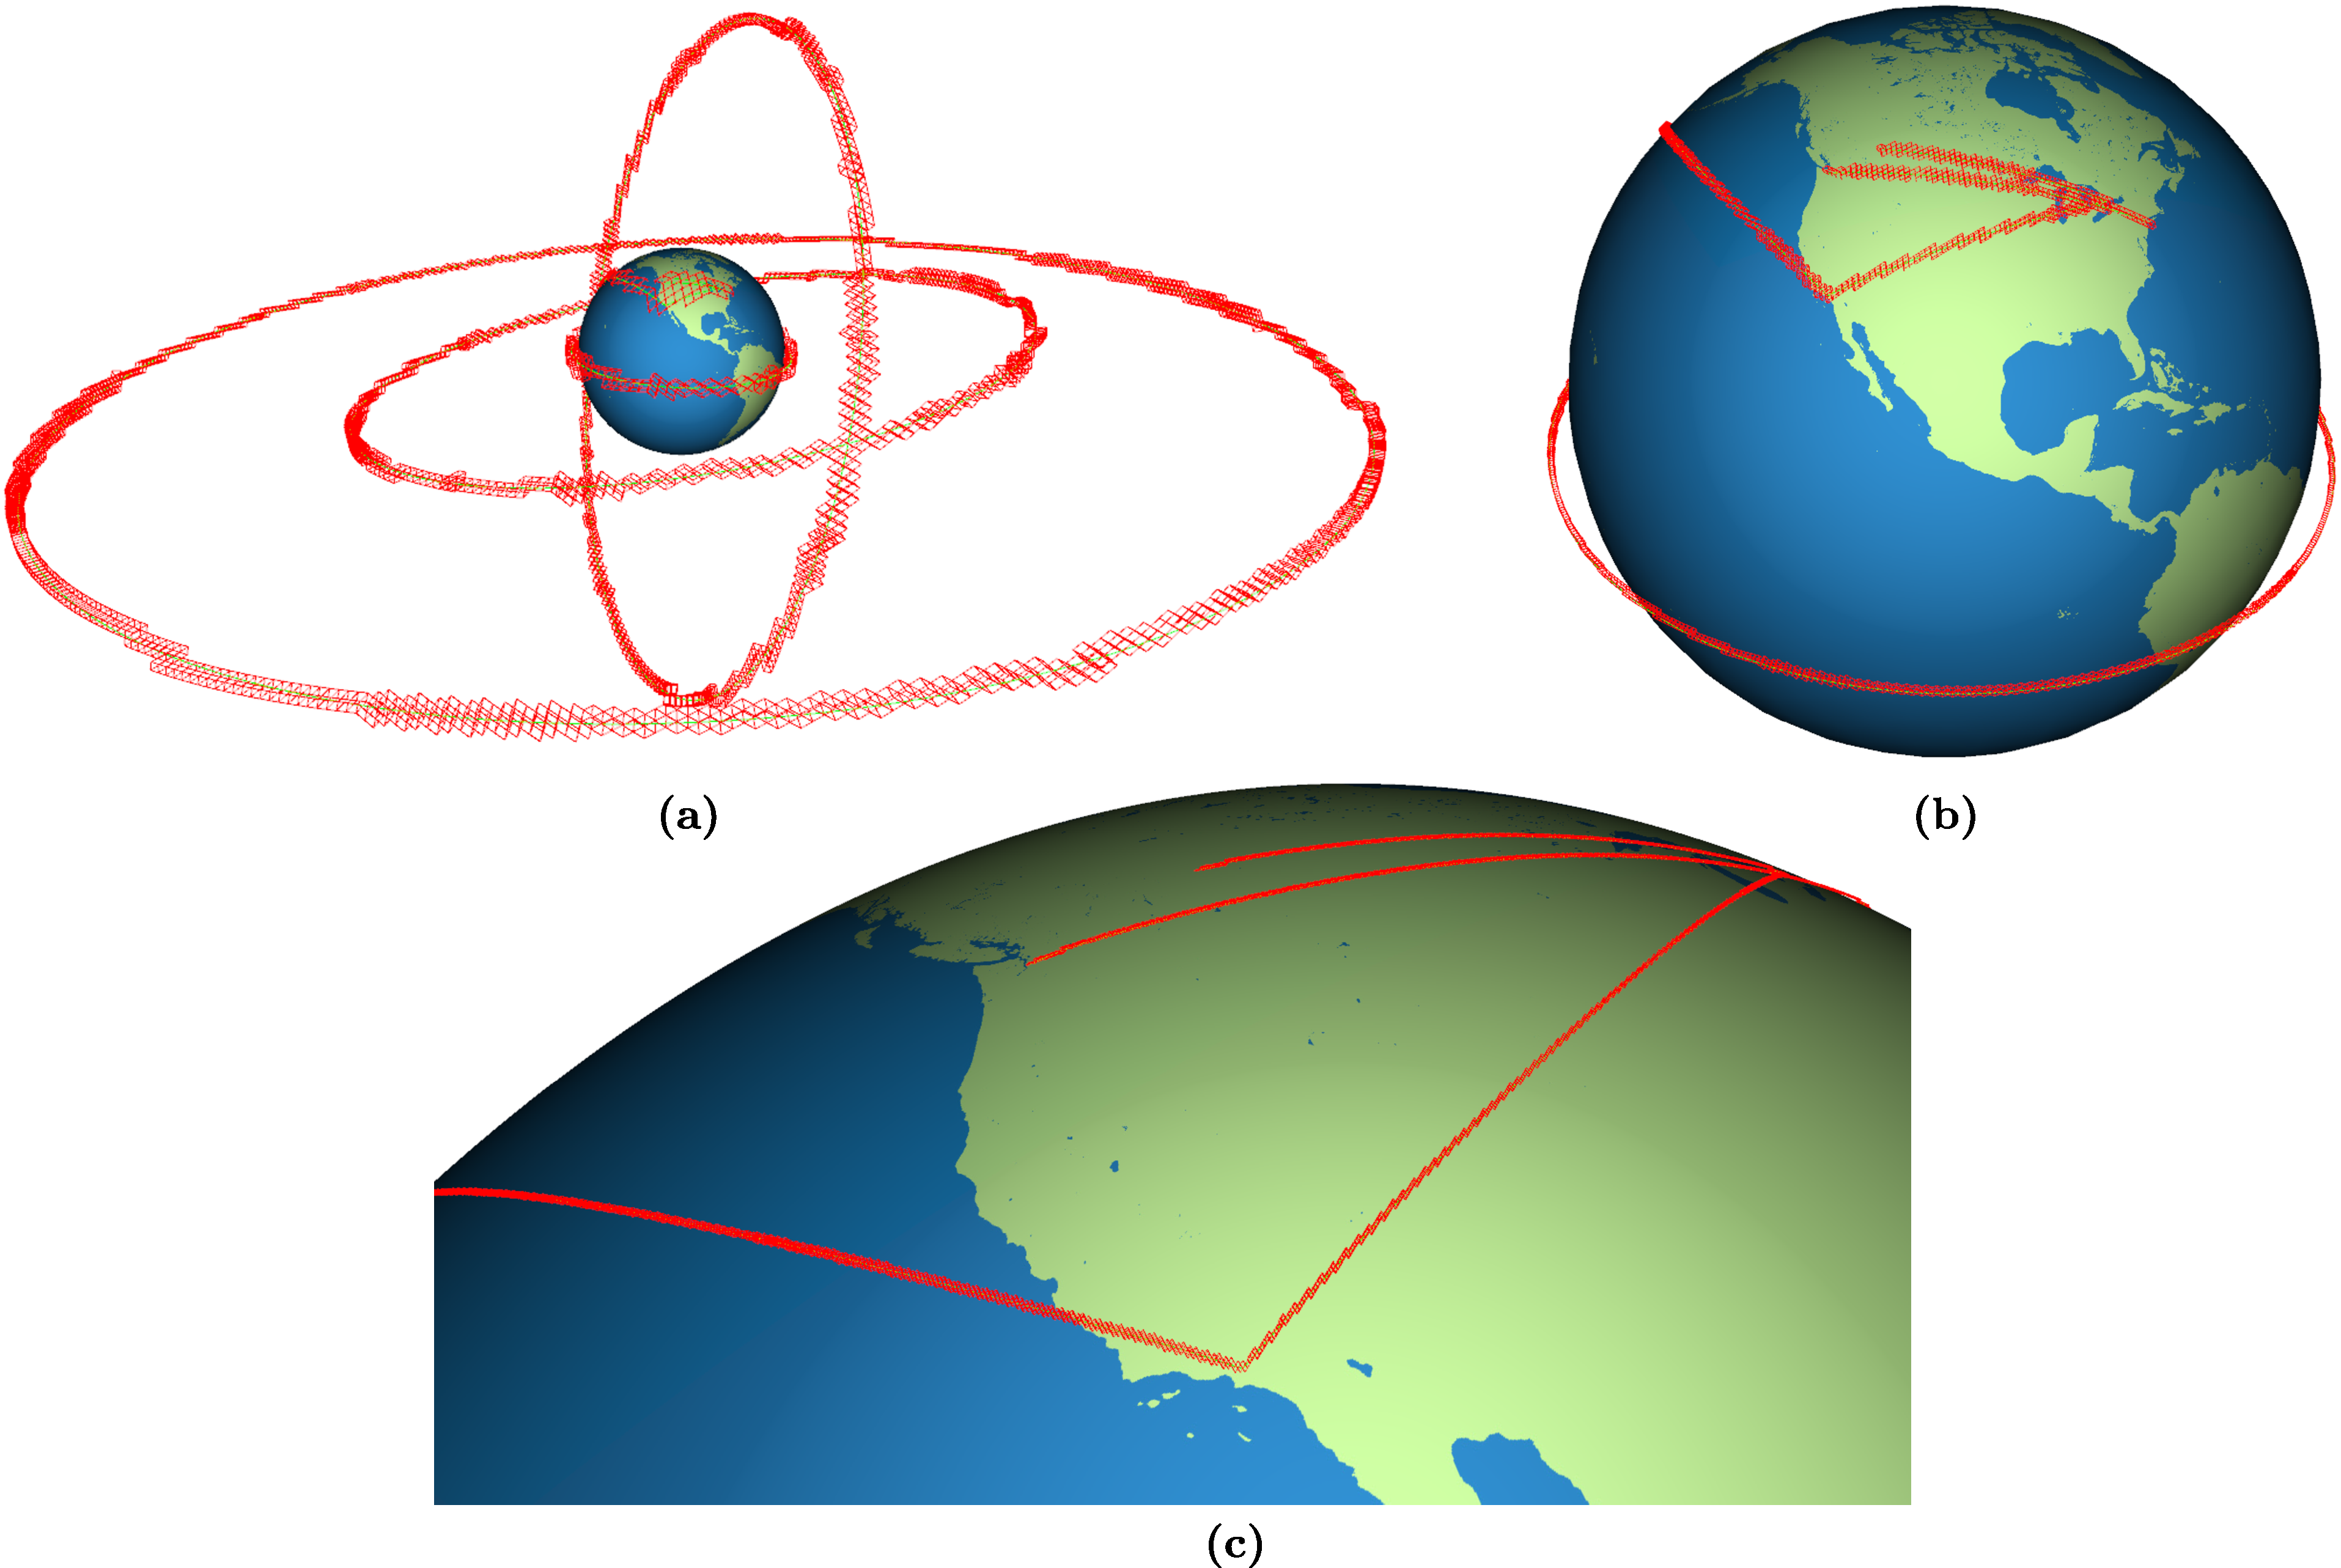
\includegraphics[width=\textwidth]{satellites.pdf}
	\caption[Flight path and satellite orbit use case showing several sample trajectories]{
		Flight paths and satellite orbits rasterized in a 3D DGGS.
		All paths and orbits are rasterized at the same grid resolution of (a) 7, (b) 10, and (c) 13.
		The width and depth of cells at these resolutions are on the order of 500~km, 100~km, and 10~km, respectively.
	}
	\label{fig:satellites}
\end{figure}


\Cref{fig:satellites} shows several flight paths and satellite orbits represented in a 3D DGGS at increasing resolutions.
The paths used in this use case are generated and do not correspond to real data.
However, the altitudes used for satellites and aircraft \text{are} accurate:
flight paths are at an altitude of 11~km (typical commercial cruising altitude); the lowest satellite is at 408~km (ISS orbit); the two middle satellites are at 20,180~km (GPS orbit); and the highest satellite is at 35,786~km (geosynchronous orbit).
The input DGGS for this example uses a rhombic triacontahedron as the initial polyhedron, regular 1:4 quadrilateral refinement, and a simple normalization projection.
The 3D DGGS has a target aspect ratio of one, a radial mapping exponent of one, and a maximum radius of 10.66$R$ (67,957~km).
These parameters were chosen to ensure that cells are relatively uniform and compact without significantly sacrificing the simplicity and efficiency of operations.


\subsection{Atmospheric Properties} \label{chap:8:atmo}
The second use case we look at is using a 3D DGGS to resample atmospheric forecasts, such as those generated by numerical weather prediction models~\cite{ncepncar, era5}.
These datasets typically have a much higher vertical resolution than surface resolution, due to how quickly properties such as temperature and wind speed tend to change in the surface versus radial dimensions.
To accommodate this difference in resolution with our 3D DGGS, we specify an appropriate aspect ratio for cells to ensure that the vertical and surface resolution matches that of the input data as closely as possible.
This use case also demonstrates how raster data is interpolated and assigned to cells in a DGGS. 


\begin{figure}[ht!]
	\centering
	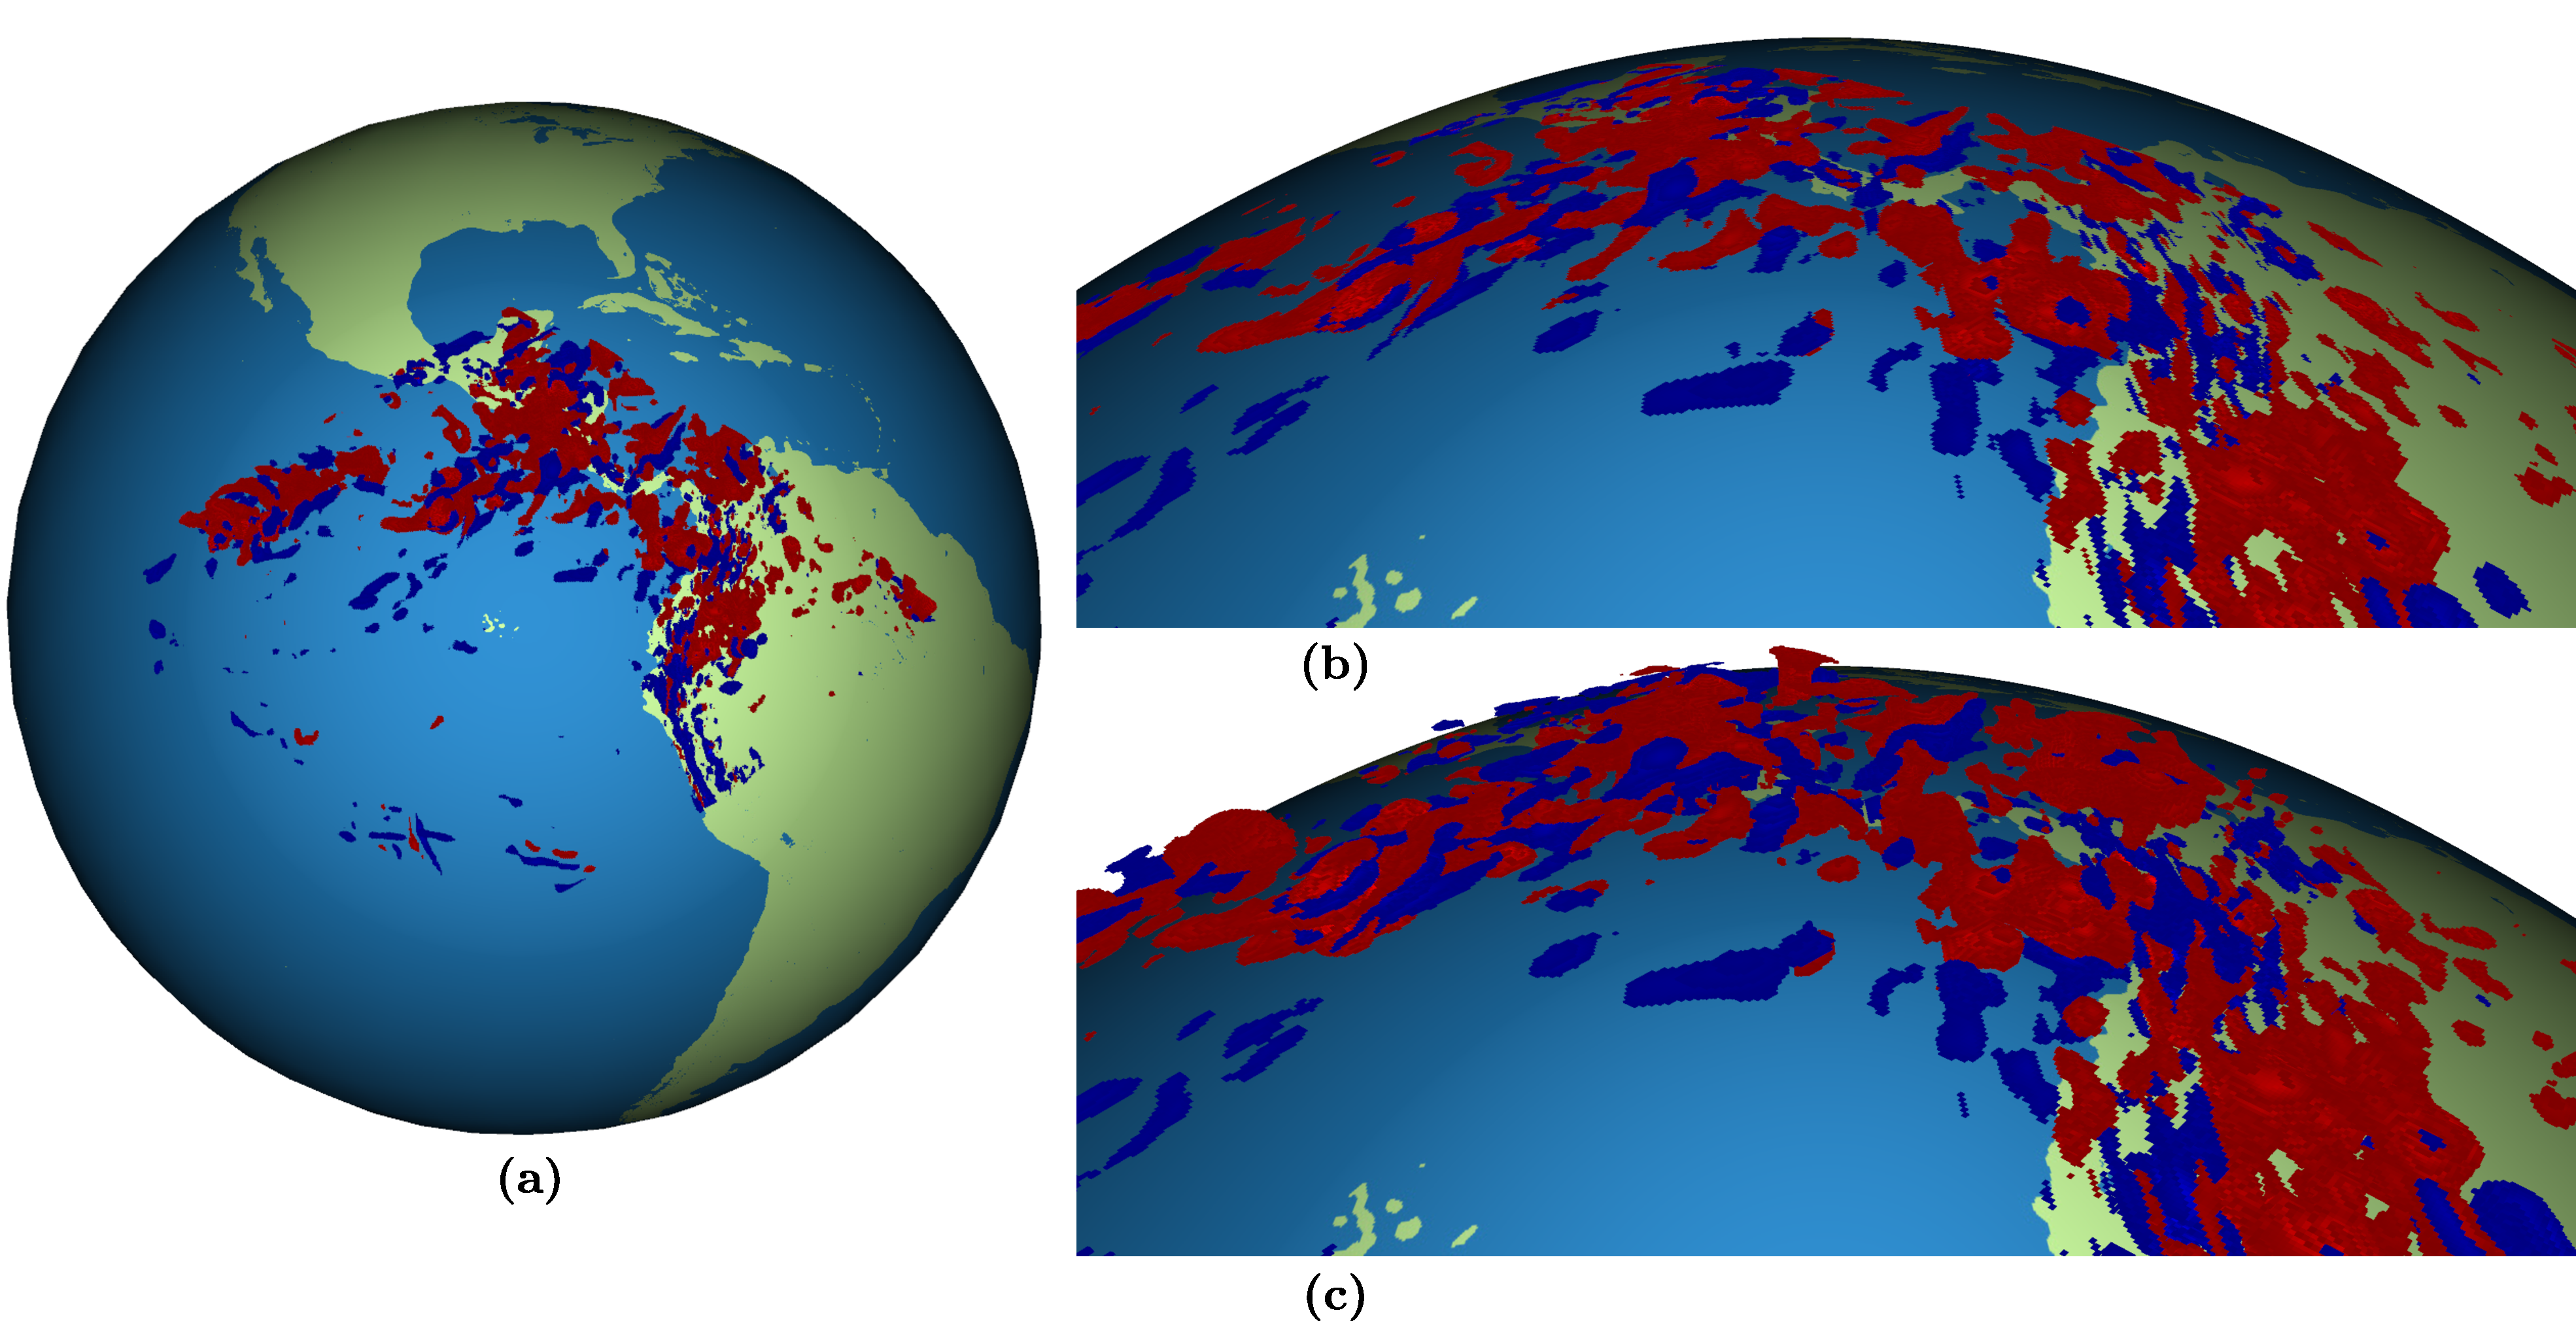
\includegraphics[width=\textwidth]{atmosphere.pdf}
	\caption[Atmospheric properties resampling use case showing vertical wind speed]{
		Vertical wind speed (mbar/s) sampled into a 3D DGGS at resolution 9.
		At this resolution, cells in the atmosphere are approximately 16~km in width and 0.5~km in depth, closely matching the resolution of the data.
		Negative velocity, which corresponds to an upward wind, is shown in red.
		Positive velocity, which corresponds to a downward wind, is shown in blue.
		Velocities with magnitude less than 0.25 mbars/s are not shown to reduce clutter and highlight regions with the highest speeds.
		In (a) and (c), altitude is scaled by a factor of 15 to better show changes in altitude; in (b), altitude is shown at its true scale.
	}
	\label{fig:atmosphere}
\end{figure}


\Cref{fig:atmosphere} shows vertical wind speed from the ERA5 dataset~\cite{era5} sampled into a 3D DGGS.
The input DGGS for this example is the same as the one used for the aircraft and satellite paths use case.
However, this 3D DGGS has a target aspect ratio of 31.7, a radial mapping exponent of one, and a maximum radius of 1.33$R$ (8495~km).


\subsection{Urban Planning} \label{chap:8:buildings}
The final use case is a volume-preserving 3D grid for urban planning and management.
A volume-preserving grid is useful for quickly estimating the volume of features rasterized in the grid by multiplying the number of cells in the raster by their shared volume.
This use case also shows the ability of our 3D DGGS to handle small scale data in addition to the much larger scale data showcased in the previous two.


\begin{figure}[ht!]
	\centering
	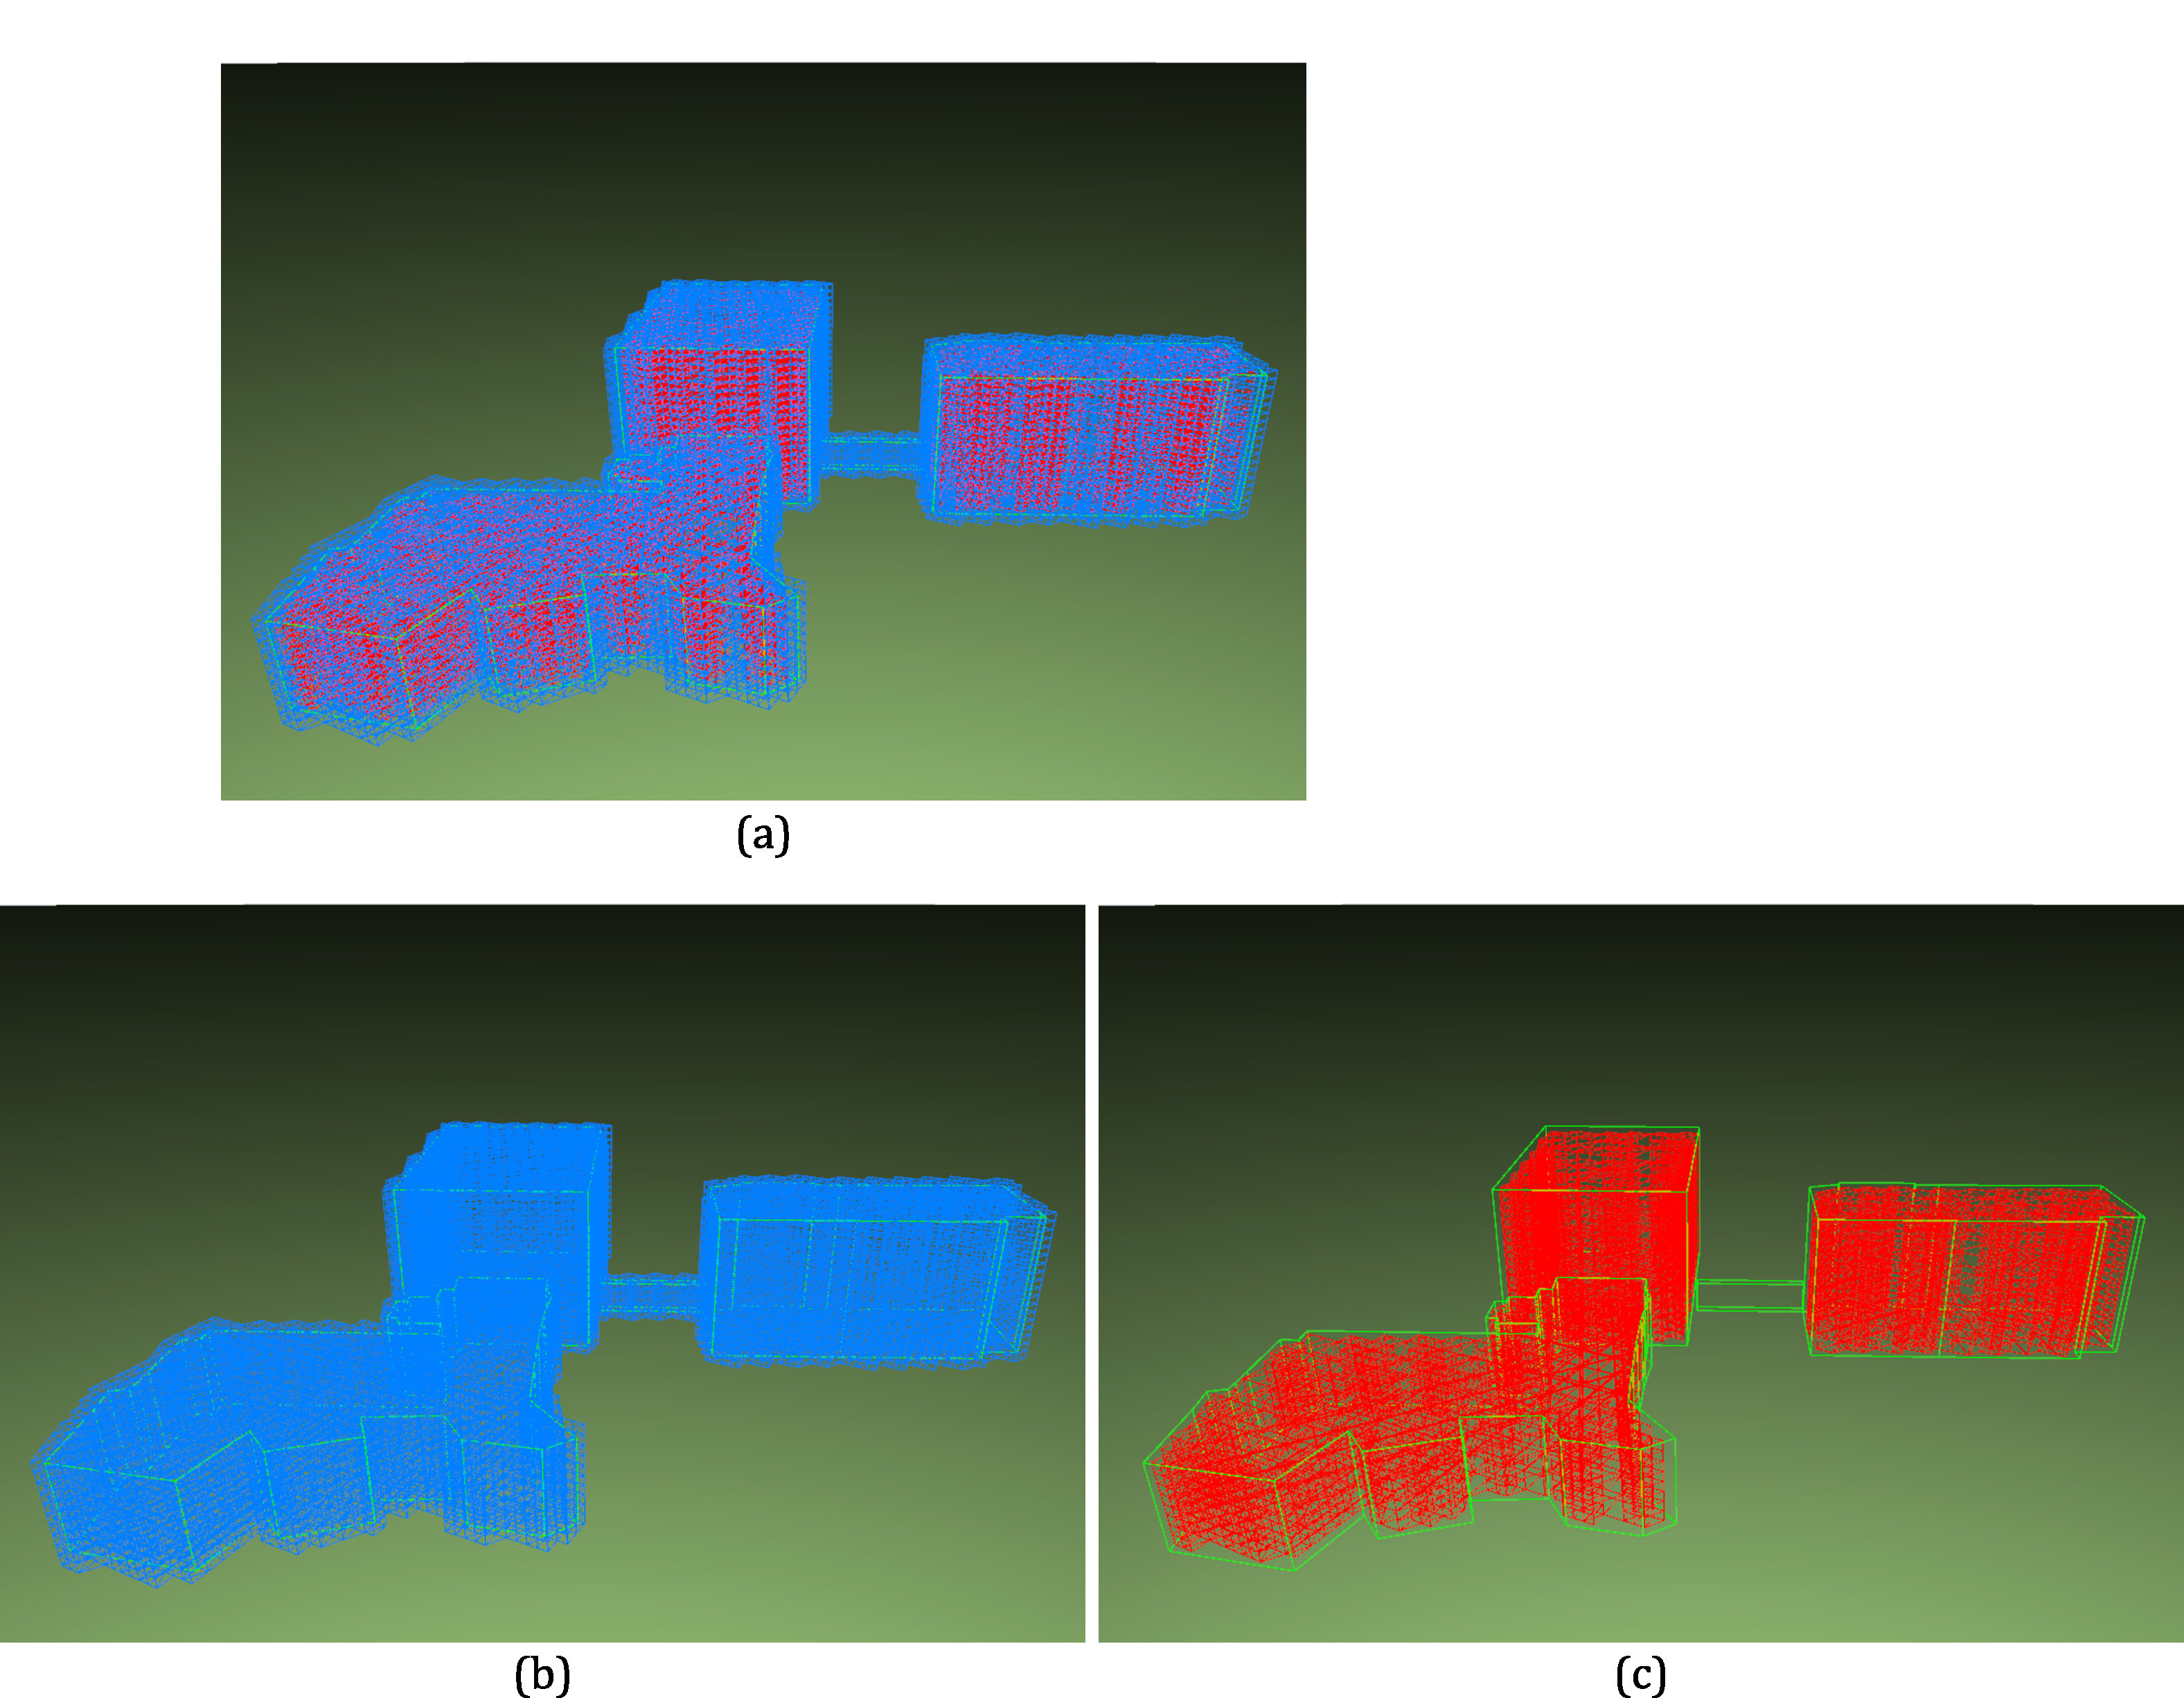
\includegraphics[width=\textwidth]{buildings.pdf}
	\caption[Urban planning use case showing various rasterized buildings]{
		A collection of buildings from the University of Calgary rasterized in a 3D DGGS at resolution 21.
		At this resolution, cells near the surface are approximately 2~m in width and depth.
		In (a), both interior and boundary cells are shown, whereas (b) and (c) show only boundary and interior cells, respectively.
	}
	\label{fig:urbanplanning}
\end{figure}


\Cref{fig:urbanplanning} shows several buildings represented in a 3D DGGS, with the building footprints obtained from Open Street Map~\cite{osm}.
To obtain full 3D geometry for the buildings, we extrude the polygon footprints vertically to create prisms; we estimate the height of the buildings as we could not find available data on this.
The input DGGS for this example is the Disdyakis Triacontahedron DGGS~\cite{hall2020disdyakis}, which uses a disdyakis triacontahedron as the initial polyhedron, a non-standard 1:4 triangle refinement, and the vertex-oriented great circle slice and dice projection~\cite{van2006slice} to preserve area.
The 3D DGGS has a target aspect ratio of one, a radial mapping exponent of three to achieve perfect volume preservation (excluding the central layer), and a maximum radius of 1.33$R$ (8495~km).


\section{Implementation} \label{chap:8:impl}
As mentioned previously, we have implemented the 3D DGGS's used in these use cases as a C++ class; this class is integrated with a research toolset used for designing and testing different conventional DGGS's.
In this toolset, the operations provided by a DGGS are specified by an abstract class that each implementation extends.
An implementation of a 2D DGGS serves as the input DGGS used during the construction of a 3D DGGS.


\Cref{fig:uml} shows a class diagram for the C++ implementation.
\textit{DGGS2D} specifies the operations that must be provided by a conventional DGGS.
It is an abstract class templated on a type to use as the index for the grid and specifies operations for encoding (pointToCell), decoding (cellToVerts), and standard indexing operations (neighbours, parents, and children).
Additionally, it provides information regarding the number of cells in the grid at a given resolution (numberOfCells) and the factor of the employed refinement (getRefinementFactor).
These are used by the 3D DGGS to obtain $n$ and $f$, respectively. QuadDGGS and TriDGGS are provided as two example \textit{DGGS2D} implementations that could exist, which use QuadIndex and TriIndex as their index types, respectively.


\begin{figure}[ht!]
	\centering
	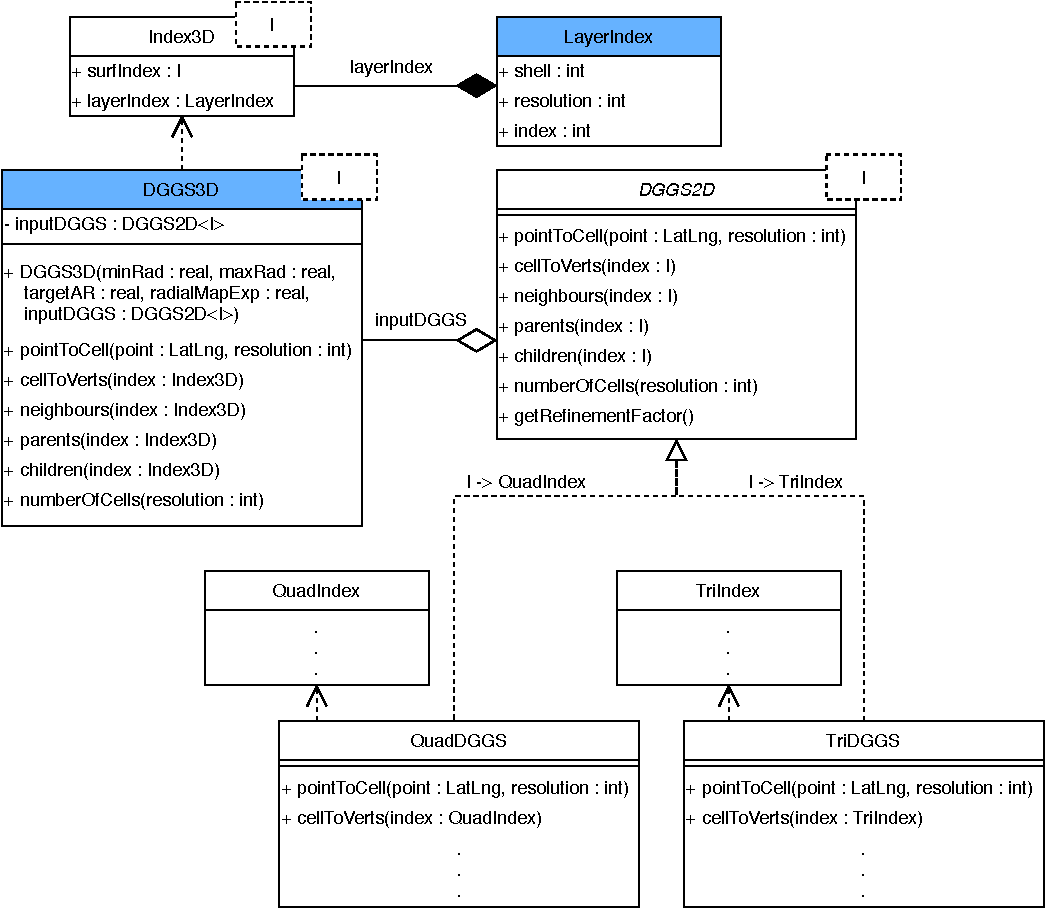
\includegraphics[width=0.95\textwidth]{3ddggs-uml.pdf}
	\caption[Class diagram of the grid extension implementation]{
		Class diagram for the implementation of our method. The classes shown in blue have their functionality described in the thesis; other classes are a part of the research toolset or otherwise support the implementation.
	}
	\label{fig:uml}
\end{figure}


During construction, a DGGS3D takes a reference to a \textit{DGGS2D} (the input DGGS) along with values maxRad ($R_\mathrm{max}$), targetAR ($a$), and radialMapExp ($t$).
This class is also templated on the type of index used by the input DGGS.
DGGS3D uses the class Index3D as its index type, which is simply a tuple composed of a surface index type and a LayerIndex.
LayerIndex is a tuple of shell ($s$), resolution ($k$), and index ($j$).
Encoding, decoding, and index operations (including mapping functions) are implemented exactly as described in \cref{chap:mapping,chap:coding}.


\section{Summary}
The above examples are only a small subset of the many potential applications of our 3D DGGS's.
Despite this, they show not only the useful properties achievable by the method (support for unbounded ranges of altitudes, volume preservation between cells, custom cell aspect ratio, and support for multiple scales of data) but also demonstrate the ease at which new 3D global grids can be created.
Given a conventional DGGS that provides the required operations, creating a 3D DGGS is as simple as providing the surface grid and three clearly defined parameters for the 3D one.
Since creating a 3D DGGS that is ideal for every application is impossible, this allows quick iterations on creating and comparing different 3D grids to find the ideal one for each application.
